%%%%%%%%%%%%%%%%%%%%%%%%%%%%%%%%%%%%%%%%%%%%%%%%%%%%%%%%%%%%%%%%%%%%%%%%%%%
\chapter{Introduction}
%%%%%%%%%%%%%%%%%%%%%%%%%%%%%%%%%%%%%%%%%%%%%%%%%%%%%%%%%%%%%%%%%%%%%%%%%%%


The Shortest Common Superstring (SCS) problem, known to be NP-Complete,
seeks the shortest string that contains all strings from a given set.
In this paper, we provide the summary of the problem and some of its characteristics.

The SCS problem has been extensively studied for its
applications in string compression and DNA sequence assembly \cite{Ma2009}.

The superstring problem has applications to data storage,
 specifically, data (string) compression \cite{Gallant1980}. 
In many programming languages, a character string may be 
represented by a pointer to that string. 
The problem for the compiler is to arrange strings 
so that they may be ``overlapped'' as much as possible.

DNA sequence assembly is another  problem to which an SCS algorithm is known to apply.
The $sequencing$ problem in molecular biology is to ``read'' a string of DNA,
which can be viewed as a string over the alphabet \{A,C,G,T\}. Sequencing produces such a large number of fragments that
almost all genome positions are covered by many fragments. This short fragments
thus have large overlaps between other pieces. Hence, they can be given as an input to SCS algorithm.
Figure \ref{fig:dna-overlap} shows an overlap graph consisting DNA reads (or fragments) as nodes. 



\begin{figure*}
\centering
\fbox{
\scalebox{0.65}{
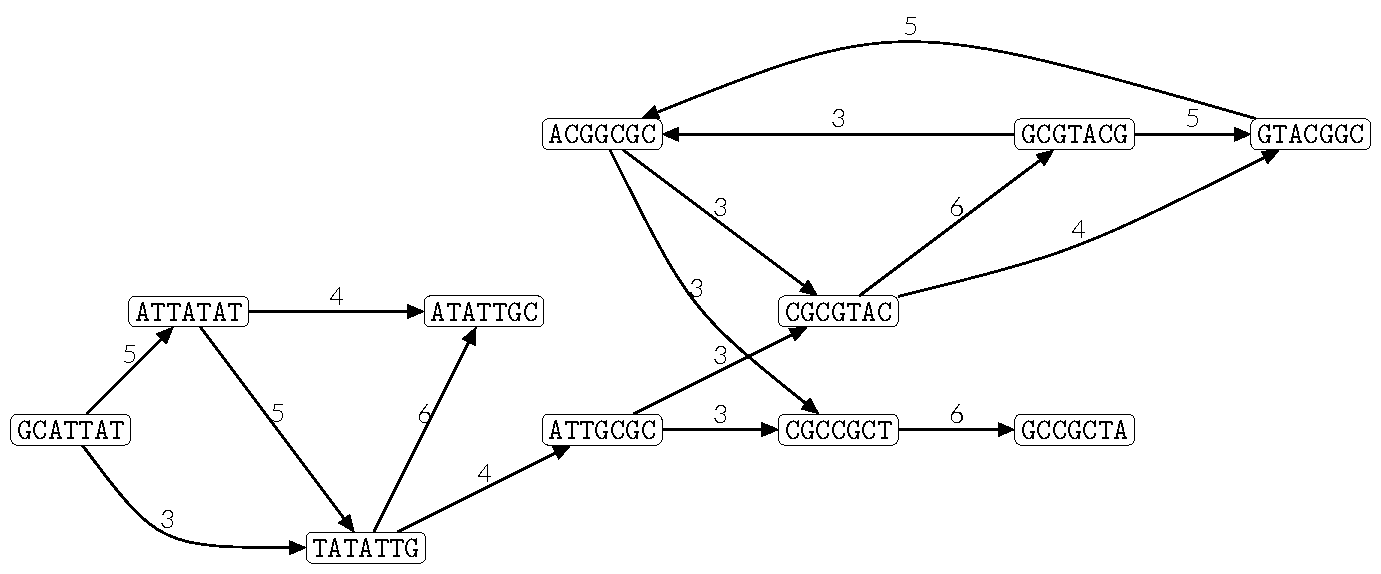
\includegraphics{fig-overlaps-dns-example}
}}
\caption{Sample overlap graph with each adjacent nodes 
having at least $k = 3$ overlaps. The original string is \texttt{GCATTATATATTGCGCGTACGGCGCCGCTACA}.}
\label{fig:dna-overlap}
\end{figure*}	

In \cite{Ma2009}'s paper, SCS was used to analyze DNA sequence assembly using
a greedy algorithm. 

\section{Project Context}

\section{Purpose and Description}

\section{Objectives}

\vfill\eject
\section{Scope and Limitations}
